%!TEX root = main_thesis.tex
%---------------------------------------------------------------------------------
\chapter{A Spectrum Efficient Shaping Method for OFDM Radios}
\label{chap:SpectralLeakage}
%---------------------------------------------------------------------------------

%---------------------------------------------------------------------------------
\section{Introduction}
\label{Sec:Intro}
%---------------------------------------------------------------------------------

This chapter is concerned with the OFDM spectral leakage challenge for OFDM-based CRs.
OFDM signals typically cause large amounts spectral leakage, whereas CRs demand a shaped spectrum confined within the allocated channel in order to reuse free spectral bands without causing ICI to other users occupying adjacent bands.
Some recent OFDM-based standards are defined with the requirements on spectral leakage that are extremely stringent in an effort  to avoid ICI.
Spectral leakage filtering may cause some effects on transmitted signals that lead to a reduction in the effective timing guard.
Therefore, the implementations of spectral leakage filtering need to be able to take into account the parameters of the underlying OFDM signal and its channel characteristics to avoid causing negative effects on the transmitted signal such as distortion and ISI.

In this chapter, a novel method that embeds baseband filtering within a cognitive radio (CR) architecture, is proposed.
The method is able to meet the specification for the most stringent 802.11p SEM, meet the specification of the 802.11af strict SEM requirement, and furthermore can allow ten additional 802.11af subcarriers to occupy a single basic channel without violating SEM specifications.
In addition, the method can adaptively change filter performance according to the transmission power to reduce computational cost while guaranteeing that the emission spectrum remains smaller than the allowed spectral leakage.
The method, performed at baseband, relaxes otherwise strict RF front-end requirements.
This allows the RF subsystem to be implemented using much less stringent 802.11a designs, which can significantly reduce total cost.

The work presented in this chapter has also been discussed in:
\begin{itemize}
\item  T. H. Pham, I. V. McLoughlin, and S. A. Fahmy, ``Shaping Spectral Leakage for IEEE 802.11p Vehicular Communications,'' in \textit{Proceedings of IEEE Vehicular Technology Conference (VTC Spring)}, Seoul, Korea, May 2014~\cite{PhamMay2014}.
\item T. H. Pham, S. A. Fahmy, and I. V. McLoughlin, ``Spectrally Efficient Emission Mask Shaping for OFDM Cognitive Radios,''  under review for \textit{IEEE Transactions on Communications (TCOM)}.
\end{itemize}

%---------------------------------------------------------------------------------
\section{Signal Model for Spectral Leakage Filtering}
\label{sec:SigMod}
%---------------------------------------------------------------------------------
Conventionally, there are two methods that can be employed to compress the spectral leakage for OFDM-based system, namely pulse shaping and image spectrum compression. Pulse shaping, recommended in 802.11a, is effective at reducing side lobes. Spectral leakage filtering is designed with respect to the signal model and channel model to avoid the negative effects of filtering. In this section, we present the OFDM signal model and 802.11p and 802.11af channel models for compressing the spectral leakage.

\subsection{Signal Model}
We define an OFDM symbol to have inverse fast Fourier transform (IFFT) length and cyclic prefix (CP) length $N$ and $N_{CP}$, respectively, so that the length of the symbol including its CP is $N_{T} = N + N_{CP}$.
A sample $x(m)$ of the OFDM symbol $(0\leq m \leq N_{T}-1)$ can be expressed in the time domain as
\begin{equation}
\label{xm}
x(m) = \frac{1}{N}\sum_{k=0}^{N-1} X(k) e^{i2\pi\frac{k}{N}(m-N_{CP})},
\end{equation}
where $X(k)$ denotes the frequency domain representation of the data subcarriers.
Since OFDM symbol samples are generally transmitted sequentially, this is equivalent to multiplying symbols with a rectangular window function, $p$.
Then the transmitted OFDM samples can be expressed as
\begin{equation}
\label{xn2}
x(n) = \frac{1}{N}\sum_{l=-\infty}^{\infty} \sum_{k=0}^{N-1} X(k) p(n-l N_{T}) e^{i2\pi\frac{k}{N}(n-N_{CP}-l N_{T}).}
\end{equation}
In a conventional OFDM system, the window function, $p(m)$, is rectangular and simply described as
\begin{equation}
\label{pm}
 p(m) =\begin{cases}1, & m = 0,1, ..., N_{T} \\  0, & otherwise \end{cases}
\end{equation}

The CIR, of length $h$, is derived from the delay spread of the channel.
If the CP is shorter than the channel delay, ISI will be present in the received symbols.
Channels experienced by the two standards discussed in this chapter will obviously differ, but both tend to experience high levels of delay spread: 802.11p because it is primarily a vehicular communications standard, and 802.11af because it operates in lower attenuation UHF and VHF bands.


The PHYs specified in 802.11p and 802.11af are largely inherited from the well-established 802.11a and 802.11ac OFDM PHYs, respectively.
The major parameters of both new PHYs are presented in Table~\ref{tab:Para}.
However, since the new standards operate in different channel regions and environments, they are subject to different, and much more stringent SEM requirements than their parent standards.
\begin{table}[h]
	\centering
	\caption{ Major parameters of 802.11p and 802.11af OFDM PHYs}
	\label{tab:Para}
	\renewcommand{\arraystretch}{1.2}
	\begin{tabular}{l|c|c|c|c}
		Parameters                      	 		& 802.11p & \multicolumn{3}{c}{802.11af} \\ \hline
		Bandwidth, MHz                  		& 10     & 6    & 7   & 8    \\ \hline
		Used subcarriers, $N_{C}$ 		& 52      & \multicolumn{3}{c}{114}      \\ \hline
		Total subcarriers, $N_{T}$  		& 64      & 144      & 168     & 144     \\ \hline
		FFT points, $N_{FFT}$      		& 64      & \multicolumn{3}{c}{128}      \\ \hline
		Subcarrier spacing $\Delta f$, MHz        	& ${10}/{64}$   & ${6}/{144}$    & ${7}/{168}$   & ${8}/{144}$   \\ \hline
		Sampling frequency, MHz			& 10 & 5.33 & 5.33 & 7.11  \\ \hline
		Fourier transform size         		& 6.4 us  & 24 us    & 24 us   & 18 us   \\ \hline
		CP length                        			& 1.6 us  & 6 us     & 6 us    & 4.5 us
	\end{tabular}
\end{table}

\subsection{802.11p Signal and Channel Models}

802.11p is defined for vehicular channels that tends to experience a larger delay spread than WLAN.
While the 802.11p symbol has 16 samples for CP (i.e. the same as in 802.11a), the guard intervals are lengthened to avoid ISI by reducing the bandwidth from 20\,MHz to 10\,MHz (i.e., a 10\,MHz sampling frequency). However this raises some challenges in the frequency domain.
First, reducing bandwidth requires a higher quality factor front-end filter circuit for the higher frequency carrier compared to 802.11a.
Second, 802.11p shares a 6 subcarrier spacing frequency guard per side with 802.11a. Given the reduced sampling frequency, this leads to the absolute frequency guard being correspondingly narrower.

Generally, vehicular communication channels with large delay spread will require an increased timing guard, hence narrowing the frequency guard, which leads to more strict filtering constraints.
Empirical channel models in \cite{Acosta-Marum2007,Sen2008} reveal how maximum delay spread varies depending on different propagation models and traffic environments.
For example, the RTV model for suburban street, urban canyon, and expressway have maximum excess delays of 700, 501, and 401\,ns, respectively~\cite{Acosta-Marum2007}.
For the V2V model, measurements in \cite{Sen2008} reveal that the 90\% largest delay spread (found in urban areas) is near 600\,ns, which is equivalent to 6 samples.
Given the fact that the CP is 16 samples, this leaves 10 samples (1~us) remaining. Any spectral leakage filtering necessary to meet the stringent SEM specification must not encroach further than this into the guard time.

\subsection{802.11af Signal and Channel Models}

On the other hand, 802.11af is defined to reuse white space in the UHF band, with three basic channel units (BCUs) of 6\,MHz, 7\,MHz, and 8\,MHz.
Within this chapter, we will confine our consideration to the narrowest (and hence possibly most problematic) 6\,MHz BCU for investigating the performance of the proposed filtering method for 802.11af.

In the 802.11af channel, the measured delay spread is less than 1\,us \cite{Lan2013}, which  is equivalent to the duration of 6 samples in the CP.
Therefore, the 802.11af guard interval of 6\,us is sufficient to avoid ISI, with the remaining 5\,us (i.e., 26 samples) being available for filtering spectral leakage, if necessary.
In the US, FCC rules mandate a very strict SEM to avoid ICI on the adjacent channels of primary users in the UHF band.
For 6\,MHz channels, the signal transmitted by TVBDs shall maintain at least 55\,dB attenuation at the edge of the channel, which is significantly higher than the requirement of the parent 802.11ac standard. In the UK, the Ofcom requirement for 8\,MHz channels is similarly strict.

%---------------------------------------------------------------------------------
\section{Related Work}
%---------------------------------------------------------------------------------

This section investigates state of the art methods from the 802.11a and 802.11ac domain, and considers their application for the newer standards.
Specifically, each method is evaluated, and shown as unsuitable in meeting the strict SEM criteria for 802.11p (and hence very unlikely to satisfy the even more stringent 802.11af SEM).

\subsection{Pulse Shaping}
\label{subsec:Pulse}
%This section investigates the possibility of using pulse shaping technique to achieve the requirement of 802.11p's SEMs.
%Pulse shaping is a technique in which a smoother transition pulse is used instead of a rectangular pulse as in conventional OFDM, resulting in compressed side lobes.
Pulse shaping (using a smooth rather than rectangular pulse), recommended in 802.11a, is effective at reducing side lobes, although it induces distortion in the subcarriers.
One way to avoid the distortion is to add extending parts, i.e. CP and cyclic suffix (CS), concatenated to the conventional OFDM symbol before the beginning and after the end respectively. The extended symbol is then multiplied with a smoothing function.
While the CP in conventional OFDM is used as a guard interval, here it is also occupied, along with the CS, for pulse shaping.

Pulse shaping extends the  $N_{T}$ length of the OFDM signal by a roll-off factor, $\beta$.
One effect of extending the symbol is to reduce spectral efficiency, and thus the CP and CS of consecutive symbols can be overlapped, as shown in Fig.~\ref{fig:PS}. This, in turn, causes ISI in the overlapped region.

In practical terms, pulse shaping using the overlapping method is effectively shortening the OFDM guard interval.
A larger $\beta$ means reduced spectral leakage, at the cost of reducing the effective guard interval since a number of guard interval samples are taken for pulse shaping.
If $\beta N_{T}$ is increased to equal the CP length, the effective guard interval is reduced to zero (i.e. there is no guard interval to prevent channel-induced ISI).
In this chapter, three state-of-the-art smoothing functions for pulse shaping are investigated. We present each in discrete form, before investigating their performance with different roll-off factors.
The first smoothing function, denoted $p_1$, is present in the IEEE~802.11a standard:

%{\small
\begin{eqnarray}
\label{p1m}
&p_1 &=\begin{cases}	sin^2( \frac{\pi}{2}(0.5+\frac{m}{2\beta N_{T}}) ), 			& 0 \leq m < \beta N_{T} \\
					 	1, 															& \beta N_{T} \leq m < N_{T}  \\
					 	sin^2( \frac{\pi}{2}(0.5-\frac{m-N_{T}}{2\beta N_{T}}) ), 	& N_{T} \leq m < (1+\beta)N_{T} \end{cases}
\end{eqnarray}
%}

The second, proposed by Bala et al.~\cite{Bala2013}, is based on a raised cosine function, denoted here as $p_2$:

%{\small
\begin{eqnarray}
\label{p2m}
&p_2 &=\begin{cases}	\frac{1}{2}+\frac{1}{2}cos(\pi(1+\frac{m}{\beta N_{T}})), 			&0\leq m<\beta N_{T} \\
					 	1, 																	&\beta N_{T}\leq m < N_{T}  \\
					 	\frac{1}{2}+\frac{1}{2}cos(\pi(1+\frac{m-N_{T}}{\beta N_{T}})),		& N_{T}\leq m<(1+\beta)N_{T} \end{cases}
\end{eqnarray}
%}

The third, denoted $p_3$, is based on the characteristics of functions with vestigial symmetry as derived by Castanheira and Gameiro~\cite{Castanheira2013}:

%{\small
\begin{eqnarray}
\label{p3m}
&p_3 &=\begin{cases}	\frac{1}{2}+\frac{9}{16}cos( \pi(1 - \frac{m}{\beta N_{T}}) ) & \\
						- \frac{1}{16}cos(3\pi(1 - \frac{m}{\beta N_{T}}) ), 					& 0 \leq m < \beta N_{T} \\
					 	1, 																	& \beta N_{T} \leq m < N_{T}  \\
					 	\frac{1}{2}+\frac{9}{16}cos( \pi \frac{m-N_{T}}{\beta N_{T}}) &\\
						-\frac{1}{16}cos(3\pi \frac{m-N_{T}}{\beta N_{T}}),					&  N_{T} \leq m < (1+\beta)N_{T} \end{cases}
\end{eqnarray}
%}

The compression of OFDM spectral side lobes as a consequence of pulse shaping is investigated by first assuming that the effect of the image spectrum caused by interpolation or digital-to-analogue conversion (DAC) is negligible.
This assumption is noted because the band gap between the desired spectrum and its image is relatively narrow.
Thus the overlapping image spectrum can influence the effectiveness of the shaped spectral leakage.
The issue will be discussed later in the chapter, where image cancellation is presented separately for 802.11p and 802.11af.

The three smoothing functions are simulated for otherwise identical channels and signals, and compared in Fig.~\ref{fig:Spec_PS}. The figure reveals the spectral envelope attenuation achieved using the three smoothing functions. %, with respect to the transmitted OFDM symbol.

\begin{figure}[t]
    \centerline{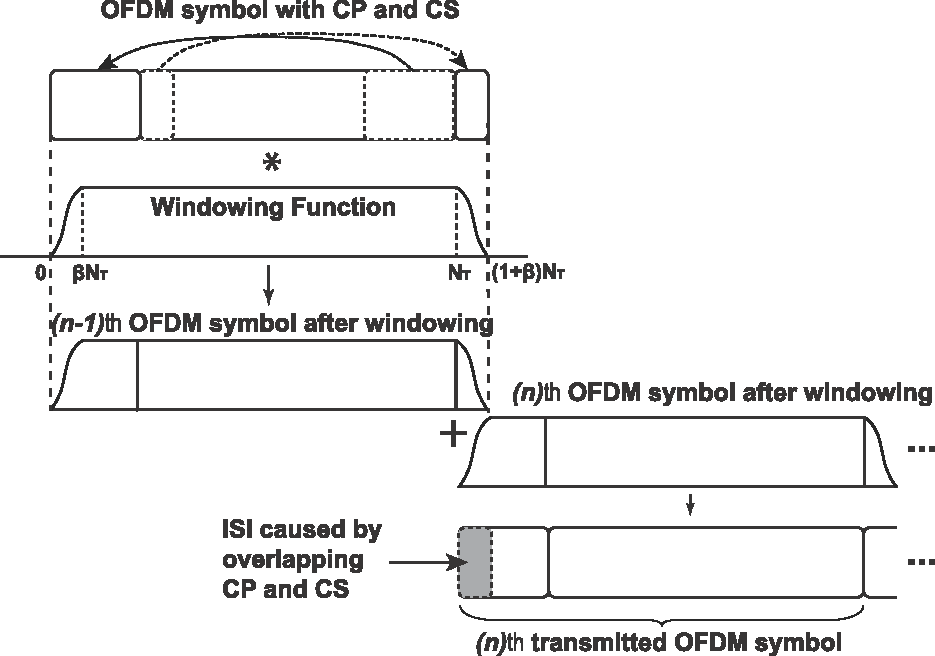
\includegraphics [width=0.9\columnwidth, height=7.5cm] {Figures/w-ofdm} }
	\vspace{-2mm}
    \caption{Pulse Shaping operation performed on OFDM symbols.}
    \label{fig:PS}
\end{figure}


\begin{figure}
	\centering
	\scalebox{1}{
	\begin{tikzpicture}
	\begin{axis}[ xlabel=Frequency (MHz), ylabel= Amplitude (dB), legend columns=3,	legend style={at={(0.5,1.02)}, anchor=south, cells={anchor=west}, draw=none}, xmin=-10, xmax=10,
	x post scale=1.4]
		\addplot+[style={dashed, color=blue}, every mark/.append style={mark=none}] coordinates
						{(-40,-50) (-15,-50) (-10,-40) (-5.5,-32) (-5,-26) (-4.5,0) (4.5,0) (5,-26) (5.5,-32) (10,-40) (15,-50) (40,-50)};
		\addlegendentry{Class C};
		\addplot+[style={dashed, color=violet}, every mark/.append style={mark=none}] coordinates
						{(-40,-65) (-15,-65) (-10,-55) (-5.5,-45) (-5,-35) (-4.5,0) (4.5,0) (5,-35) (5.5,-45) (10,-55) (15,-65) (40,-65)};
		\addlegendentry{Class D};
		\addplot+[black, style={solid, color=gray}, every mark/.append style={mark=none}]  table [x index=0, y index=1] {./Dat/PulseshapeM10.dat};
		\addlegendentry{os};
		\addplot+[black, style={dotted, color=blue, thick}, every mark/.append style={mark=none}]	 table [x index=0, y index=2] {./Dat/PulseshapeM2.dat};
		\addlegendentry{$p_1\_\beta$1};
		\addplot+[black, style={dotted, color=violet, thick}, every mark/.append style={mark=none}]  table [x index=0, y index=3] {./Dat/PulseshapeM2.dat};
		\addlegendentry{$p_2\_\beta$1};
		\addplot+[black, style={dotted,  color=red, thick}, every mark/.append style={mark=none}]	 table [x index=0, y index=4] {./Dat/PulseshapeM2.dat};
		\addlegendentry{$p_3\_\beta$1};
		\addplot+[black, style={solid, color=blue, thin}, every mark/.append style={mark=none}]	 table [x index=0, y index=2] {./Dat/PulseshapeM10.dat};
		\addlegendentry{$p_1\_\beta$5};
		\addplot+[black, style={solid, color=violet, thin}, every mark/.append style={mark=none}]  table [x index=0, y index=3] {./Dat/PulseshapeM10.dat};
		\addlegendentry{$p_2\_\beta$5};
		\addplot+[black, style={solid, color=red, thin}, every mark/.append style={mark=none}]	 table [x index=0, y index=4] {./Dat/PulseshapeM10.dat};
		\addlegendentry{$p_3\_\beta$5};
	\end{axis}
%	\end{semilogyaxis}
	\end{tikzpicture}
	}
\caption{Spectral envelope due to pulse shaping OFDM symbols using three smoothing functions and different roll-off factors for 802.11p. Class C and D spectral emission mask limits are overlaid as dotted lines.}
\label{fig:Spec_PS}
\vspace{-4mm}
\end{figure}
%
In Fig.~\ref{fig:Spec_PS}, \emph{os} shows the original OFDM spectrum without applying pulse shaping.
$p_1\_\beta1$, $p_2\_\beta1$, $p_3\_\beta1$ show the spectra of the OFDM signal using smoothing functions $p_1(m)$ to $p_3(m)$, respectively, and roll-off factor $\beta N_{T}=1$. Plots are also shown for the same functions with roll-of factor $\beta N_{T}=5$.
In the case of using one guard interval sample, the spectral leakage is reduced compared to the original OFDM signal, and  $p_1(m)$ obtains better results than the other two methods, however, the shaped spectra do not meet the emission requirement of class C.
When 5 CP samples are used for pulse shaping, $p_2(m)$ and $p_3(m)$ achieve a significant improvement, and in fact, $p_2\_\beta5$ satisfies class C and almost meets the requirement of class D.

Thus, we can state that, ignoring the presence of an image spectrum as noted previously, the pulse shaping method can take part of the guard interval to apply a smoothing function in order to shape the spectral leakage and nearly meet  stringent SEM requirements.

\begin{figure}
	\centering
	\scalebox{1}{
	\begin{tikzpicture}
	\begin{axis}[ xlabel=Frequency (MHz), ylabel= Amplitude (dB), legend columns=3,	legend style={at={(0.5,1.02), thick}, anchor=south, cells={anchor=west}, draw=none}, xmin=-10, xmax=10,
	x post scale=1.4]
		\addplot+[style={dashed, color=blue}, every mark/.append style={mark=none}] coordinates
						{(-40,-50) (-15,-50) (-10,-40) (-5.5,-32) (-5,-26) (-4.5,0) (4.5,0) (5,-26) (5.5,-32) (10,-40) (15,-50) (40,-50)};
		\addlegendentry{Class C};
		\addplot+[style={dashed, color=violet}, every mark/.append style={mark=none}] coordinates
						{(-40,-65) (-15,-65) (-10,-55) (-5.5,-45) (-5,-35) (-4.5,0) (4.5,0) (5,-35) (5.5,-45) (10,-55) (15,-65) (40,-65)};
		\addlegendentry{Class D};
		\addplot+[black, style={solid, color=lightgray}, every mark/.append style={mark=none}]  table [x index=0, y index=1] {./Dat/PulseshapeM10_inter.dat};
		\addlegendentry{os};
		\addplot+[black, style={solid, color=green}, every mark/.append style={mark=none}]	 table [x index=0, y index=2] {./Dat/PulseshapeM10_inter.dat};
		\addlegendentry{ps1\_$\beta$5};
		\addplot+[black, style={solid, color=red}, every mark/.append style={mark=none}]  table [x index=0, y index=3] {./Dat/PulseshapeM10_inter.dat};
		\addlegendentry{ps2\_$\beta$5};
		\addplot+[black, style={solid,  color=black}, every mark/.append style={mark=none}]	 table [x index=0, y index=4] {./Dat/PulseshapeM10_inter.dat};
		\addlegendentry{ps2\_$\beta$5};
	\end{axis}
	\end{tikzpicture}
	}
\caption{Spectrum of 802.11p OFDM symbols shaped with different window functions, with the image spectrum included.}
\label{fig:Inter_Spec_PS}
\vspace{-4mm}
\end{figure}

To investigate further, Fig.~\ref{fig:Inter_Spec_PS} plots simulation results for pulse shaped 802.11p OFDM symbols with the presence of the image spectrum included.
The image is a consequence of interpolation or DAC response.
The plot shows that pulse shaping yields a response that is similar to, but slightly better than, the original OFDM signal.
However, when the image spectrum is considered, pulse shaping clearly can not achieve meaningful adjacent channel signal compression.
In fact, the band gap between the main spectrum and the image spectrum is insufficient for pulse shaping to achieve any significant spectral leakage decay.

In a practical system, the consequence is that almost all of the side-lobe attenuation may need to be contributed by sharp and hence both high order and accurate analogue filters.
Such filters contribute design complexity, increased component count, manufacturing difficulty, and additional cost to a product.

\subsection{Image Spectrum Cancellation By FIR Filter}
\label{subsec:FIR}
The critical issue for 802.11p signals to meet the stringent mask requirements is that the frequency guards are narrow and the carrier frequency is relatively high (5.9\,GHz) compared to 802.11a.
Similarly, the 802.11af guard bands are even narrower, and the sub-channels are also much narrower.
Interpolation can be used at baseband to increase sampling frequency, and thereby expand the baseband bandwidth.
This then provides a wider frequency transition band, which is easier to fit a filter roll-off response into, however the resulting image spectra (repeats of the original baseband spectrum) must then be removed by filtering.
%, commonly implemented as an FIR filter, may be used to cancel image spectra.
Such filters are commonly implemented using finite impulse response (FIR) form.
A cascaded integrator comb (CIC) implementation is sometimes chosen, since this can combine the interpolation and filtering steps, however while it is computationally efficient it lacks flexibility,
Since this chapter is concerned with the tradeoff between the filter order, duration of impulse response, degree of oversampling, and filter transition band sharpness, flexibility is important and thus general FIR form filters are assumed.

The tradeoff mentioned above exists because the narrow band gap between main and adjacent image spectra mandates a high order filter to remove ICI, which generally implies a high order and thus long impulse response filter.
Unfortunately the long impulse response of the filter has a similar effect to the impulse response of the overall channel in terms of inducing ISI.
Thus the FIR filter also reduces the effective guard interval of OFDM symbols~\cite{farhang2008signal}.
Consequently, its design must contribute to the wider tradeoff between ISI avoidance, spectral efficiency (the transition band width), and degree of filter attenuation needed to meet the SEM requirement.

Several widely used FIR implementation filters are listed in Table~\ref{tab:lengthFIR}. These are all be investigated for image spectrum attenuation, as applied to 802.11p symbols initially, and then evaluated for 802.11af.
%The table lists their attenuation, and length (in taps) in the first two columns.
An empirical formula~\cite{Kapadia2012} is used to estimate the length of each filter in terms of attenuation $A$ and transition band $\Delta\omega$.
The specifications of the stringent 802.11p class D SEM are used to calculate the required number of taps with L-fold interpolation, in terms of L.

\begin{table}[h]
	\centering
	\caption{Popular window-based FIR filter lengths}
	\label{tab:lengthFIR}
	\renewcommand{\arraystretch}{1.5}
	\begin{tabular}{@{}lp{2cm}p{3.4cm}p{2.5cm}@{}}
       \toprule
    		  Window 	& Stopband Attenuation  & Filter Length, N   & Length for 802.11p\\
    	\midrule
		Hamming, 	$HM$		& $-26.5$dB	& $\frac{6.22\pi}{\Delta\omega}$							&  $N \approx 31 L$ \\
		Hanning, $HN$				& $-31.5$dB	& $\frac{6.65\pi}{\Delta\omega}$							&  $N \approx 33 L$ \\
		Backman, $BM$			& $-42.7$dB	& $\frac{11.1\pi}{\Delta\omega}$							&  $N \approx 55 L$ \\
[1ex]		Kaiser, $KS$				& --- 		&\parbox{3cm}{	$\frac{A-7.95}{2.23 \Delta\omega}, A>21$ \\
[1ex]												$\frac{5.79}{\Delta\omega}, A<21$}			& $N \approx 33 L$ \\
[1ex]		Chebyshev, $CW$		      & ---		& $\frac{2.06A -16.5}{2.29 \Delta\omega}$					& $N \approx 67 L$ \\
    	\bottomrule
    \end{tabular}
\end{table}

It is noticeable that the required lengths of these FIR filters for 802.11p are all longer than the 1.6\,us guard interval of the 802.11p symbol.
For example, the Hanning window requires filter length $N \approx 33\times L$ samples (each sample duration is $\frac{1}{L.10MHz}$ ), equivalent to a duration of 3.3~us.
%Thinh: I added "1.6us" above... is that correct? How did you compute the filter time in us? Is this example correct: if N=33L and each sample duration is L/10MHz then the duration is 3.3us}
To avoid ISI, the maximum length of the FIR filter is derived by taking into account the guard interval and the CIR.
By assuming that the delay spread of the vehicular channel is constrained to a maximum of 600~ns (as discussed in Section~\ref{sec:SigMod}) based on the results stated in \cite{Acosta-Marum2007,Sen2008}, the CIR is equivalent to 6 samples of the 802.11p guard interval (the sampling frequency of 802.11p is 10\,MHz).
Therefore, a remaining effective guard interval of 10 samples is available for filtering.
However, when the filter is used in a transmitter, a matched filter is required at the receiver~\cite{farhang2008signal} with equivalent length, meaning that the remaining guard interval is effectively halved: only 5 samples remain for transmitter filtering.

Given that L-fold interpolation is used at the transmitter, the permitted FIR filter length becomes $5 \times L$, constituting one of the rules for the FIR filter design process.

Theoretically, in the conventional approach, a value of $L$ can be chosen based on the baseband sampling frequency ($F_s=$10\,MHz for 802.11p) and the DAC maximum frequency, $F_{DAC}^{max}$, such that $F_{DAC}=L.F_s \le F_{DAC}^{max}$.

In the proposed method, the baseband frequency of the OFDM symbol is increased by a factor of $M$ over the critical sampling frequency (where $M$ is a power of two). Thus, to maintain the same DAC sampling frequency, $F_{DAC}=L'\cdot M\cdot Fs$, only $L'$-fold interpolation is required.
It is clearly preferable that $L'/M$ is an integer.
For comparison between the proposed and conventional approaches, $L$ should also be an integer, and in this chapter, assuming $F_{DAC}^{max}$=80\,MHz, we choose $L=8$ for the conventional method, and compare with two values of $L'$ ($2$ and $4$).

\begin{figure}
	\centering
	\scalebox{1}{
	\begin{tikzpicture}
	\begin{axis}[ xlabel=Frequency (MHz), ylabel= Amplitude (dB), legend columns=4,	legend style={at={(0.5,1.02, ultra thick)}, anchor=south, cells={anchor=west}, draw=none}, xmin=-20, xmax=20,
	x post scale=1.4]

		\addplot+[style={dashed, color=black}, every mark/.append style={mark=none}] coordinates
						{(-40,-40) (-15,-40) (-10,-28) (-5.5,-20) (-5,-10) (-4.5,0) (4.5,0) (5,-10) (5.5,-20) (10,-28) (15,-40) (40,-40)};
		\addlegendentry{Class A};
		\addplot+[style={dashed, color=green}, every mark/.append style={mark=none}] coordinates
						{(-40,-40) (-15,-40) (-10,-28) (-5.5,-20) (-5,-16) (-4.5,0) (4.5,0) (5,-16) (5.5,-20) (10,-28) (15,-40) (40,-40)};
		\addlegendentry{Class B};
		\addplot+[style={dashed, color=blue}, every mark/.append style={mark=none}] coordinates
						{(-40,-50) (-15,-50) (-10,-40) (-5.5,-32) (-5,-26) (-4.5,0) (4.5,0) (5,-26) (5.5,-32) (10,-40) (15,-50) (40,-50)};
		\addlegendentry{Class C};
		\addplot+[style={dashed, color=violet}, every mark/.append style={mark=none}] coordinates
						{(-40,-65) (-15,-65) (-10,-55) (-5.5,-45) (-5,-35) (-4.5,0) (4.5,0) (5,-35) (5.5,-45) (10,-55) (15,-65) (40,-65)};
		\addlegendentry{Class D};

		\addplot+[smooth, style={solid, color=green, thin}, every mark/.append style={mark=none}]	 table [x index=0, y index=2] {./Dat/filtered_spec.dat};
		\addlegendentry{KS};
		\addplot+[smooth, style={solid, color=cyan, thin}, every mark/.append style={mark=none}]  table [x index=0, y index=3] {./Dat/filtered_spec.dat};
		\addlegendentry{HM};
		\addplot+[smooth, style={solid, color=red, thin}, every mark/.append style={mark=none}]	 table [x index=0, y index=4] {./Dat/filtered_spec.dat};
		\addlegendentry{HN};
		\addplot+[smooth, style={solid, color=blue, thin}, every mark/.append style={mark=none}]	 table [x index=0, y index=5] {./Dat/filtered_spec.dat};
		\addlegendentry{BM};
		\addplot+[smooth, style={solid, color=black, thin}, every mark/.append style={mark=none}]	 table [x index=0, y index=7] {./Dat/filtered_spec.dat};
		\addlegendentry{CW};
	\end{axis}
	\end{tikzpicture}
	}
	\vspace{-2mm}
\caption{Spectra of OFDM symbols for 802.11p using different FIR interpolation filters, with $L=8$.}
\label{fig:FirSpec}
\vspace{-4mm}
\end{figure}

To visualise the spectral performance, a simulation is performed, with $L=8$, to evaluate filtered spectra using each window function, for 802.11p symbols.
The spectral responses are plotted in Fig.~\ref{fig:FirSpec}, where the same OFDM signal as in Fig.~\ref{fig:Inter_Spec_PS} has been filtered by the FIR interpolation filters, and compared to the SEMs.
In the figure, the filtered spectra obtained by using Kaiser, Hamming, Hanning, Blackman, and Chebyshev windows are compared (denoted using the abbreviations in Table~\ref{tab:lengthFIR}).
In each case, two prominent auxiliary peaks, visible beside the main spectrum, are the biggest impediments to satisfying the SEM criteria.
In detail, the Blackman filtered spectrum slightly exceeds the class A limits, whereas the remaining filters are able to meet the requirements of classes A and B but not of classes C and D. In fact, none of the filters are even close to class C and D compliance.
Hence, given the effective guard interval of 802.11p, FIR filtering clearly does not provide a solution.

The simulation results show that the common filtering methods used at interpolated baseband are not even close to meeting the strict SEM requirements of 802.11p.
Although not shown here, this is of course equally true of the more stringent 802.11af SEM.
This result implies that 802.11p and 802.11af implementations must rely on sharp front end RF and analogue filtering, which typically results in an increased total system cost and reduced power efficiency.

%---------------------------------------------------------------------------------
\section{Proposed Spectrum Efficient Shaping Method}
%---------------------------------------------------------------------------------
The discussions above have revealed that the main challenge to conforming with strict SEMs is the narrow frequency guard which must accommodate a very sharp filter transition between pass and stop bands, since the stop-band attenuation is high.
In this section, we briefly explain the method before building upon its foundation to derive a CR architecture for OFDM spectral leakage mitigation which we will then evaluate for both 802.11p and 802.11af.

\subsection{New Spectral Leakage Filtering Method}

In a conventional approach, pulse shaping is only employed with small roll-off factors.
This is because large roll-off factors involve longer filters, reducing the effective guard interval.
Given the narrow frequency guard of the OFDM spectrum for the new standards, and the amount left after accounting for the effects of CIR and matching filters, pulse shaping under such constraints is unable to cancel the image spectrum: in fact, even if the entire guard interval was to be used, this may be insufficient for the very stringent class D SEM in 802.11p, and the SEM of 802.11af.
Thus our new method takes a different approach.
Instead of using a large proportion of the guard interval for FIR filtering, we allow the pulse shaping to occupy a significant portion of the guard space, with large roll-off factors.
To obtain the significant spectral leakage reduction necessary, the frequency guard needs to be increased.
It thus involves introducing a frequency guard extension technique.
Then, given a wider frequency guard, pulse shaping with large roll-off factors can achieve significant side lobe compression of the OFDM signal, and the required transition band for FIR filtering is extended, which means a shorter FIR filter is able to attenuate the image spectrum.

The method thus involves three steps:

\begin{itemize}
\item The IFFT length is multiplied by a factor $M$, and the sampling frequency similarly increased by a factor $M$, to maintain the same subcarrier spacing.
Given this, the allocation vector is formed to add data symbols at lower subcarriers that are the same as those in the original IFFT, while the remaining subcarriers are zero-padded.
\item Next, pulse shaping is applied in the normal way, to meet the given SEM constraint.
\item Finally, $L'$-fold interpolation is used to allow simple filtering to remove the image spectrum.
\end{itemize}

Based on the proposed approach, we build a flexible CR architecture which is demonstrated to achieve the SEM requirements for both 802.11p (all classes A, B, C and D) as well as 802.11af in the UHF band.

\subsection{Novel CR Filtering Architecture}

A CR architecture for OFDM implies the agility to handle non-contiguous (NC) transmission of symbols (NC-OFDM) as well as the ability to adapt to different frequency bands, bandwidths and timing synchronisation regimes.
For the purposes of this chapter, a CR architecture is developed which combines  transmission of NC-OFDM symbols with switched sampling frequency, supporting both 802.11p and 802.11af.
In particular, the architecture adaptively extends the frequency guard as required, and performs both pulse shaping and FIR interpolation filtering to meet the most strict SEM requirements of both standards.
It should be understood that this CR architecture is designed to demonstrate compliance with the more difficult standards: it could trivially be de-rated to the much less stringent 802.11a and 802.11ac parent standards.

The proposed CR-based transmitter architecture structure is presented in Fig.~\ref{fig:Struc}, as implemented on a Xilinx FPGA for experimental purposes.
\begin{figure}[t]
    \centerline{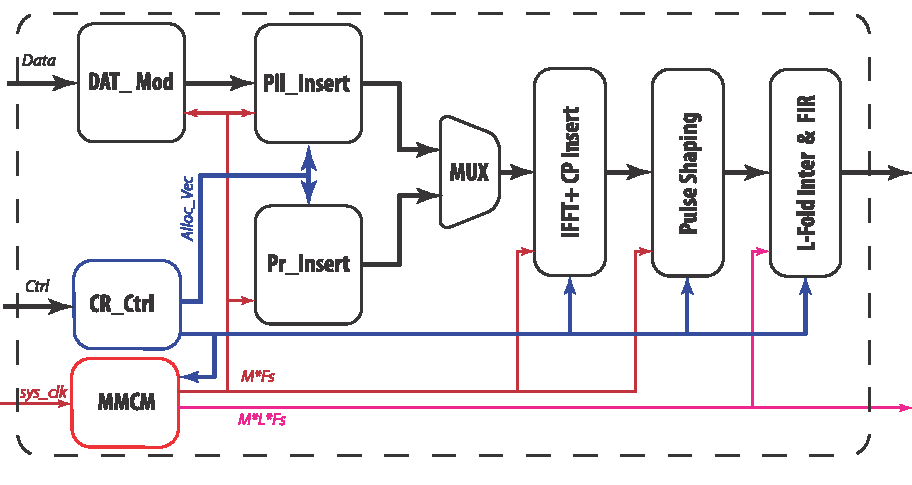
\includegraphics [width=0.9\columnwidth] {Figures/CRTx_shaping} }
	\vspace{-2mm}
    \caption{The CR-Based architecture for adaptive OFDM spectral leakage shaping.}
    \label{fig:Struc}
\end{figure}
As can be seen, the architecture consists of the baseband sub-modules, including %data modulation ($DAT_Mod$), pilot insertion ($Pil_Insert$), preamble insertion ($Pr_Insert$), IFFT and CP adding ($IFFT+CP insert$), $Pulse shaping$, L-fold interpolation and FIR filtering ($L-Fold Inter \& FIR$).
\emph{Pil\_Insert} which flexibly inserts data symbols and pilots from the data modulator, \emph{DAT\_Mod}, into an OFDM symbol according to the current allocation vector (\emph{Alloc\_Vec}).
\emph{Pre\_Insert} inserts the preamble symbol while \emph{IFFT+CP Insert} is an IP core that with flexibly reconfigurable IFFT length and CP insertion.
\emph{PulseShaping} performs pulse shaping with a smoothing function for which the roll-off factor can be changed from small, for relaxed spectral shaping, to large, for more stringent spectral shaping.
\emph{L-Fold Inter\&FIR} performs $L'$-fold interpolation, with $L'$ being controllable on a symbol-by-symbol basis. After interpolation, the FIR block is used to filter out the image spectrum.
In addition, for the CR architecture, the cognitive control sub-module (\emph{CR\_Ctrl}) is used to modify sub-module parameters to match SEM requirements imposed from the higher layers (i.e.\ it adjusts timing, bandwidth, frequency band and SEM requirements).
The mixed-mode clock manager (\emph{MMCM}) is another integrated IP core used to manage the sampling clock ($\mathit{F_s}$), which is set according to the filter performance requirements and operating frequency band.

In addition, the \emph{MMCM} allows the transmitter to reduce the degree of filtering (i.e. degree of spectral leakage shaping) when transmission power is reduced: since transmit power reduction naturally reduces ICI.
This is particularly important for lower power operating modes in which a lower sampling frequency, less filtering complexity, and reduced transmission amplitude all contribute to power savings.

Compare this with the 802.11p prototype presented in \cite{Choi2014}, which was adopted for direct device-to-device communication between smartphones.
That innovative prototype was able to adaptively increase transmission power to extend communication range.
However, the system was based on an 802.11a hardware solution and baseband, and did not investigate the increased spectral leakage when the transmitted signal was amplified to increase range (at which point it would not be likely to meet the 802.11p SEM requirement).

By contrast, the method proposed and implemented in this chapter, is able to apply a more stringent SEM filter when transmission power is increased such that ICI exceeds a given threshold.
In particular, \emph{CR\_Ctrl} is invoked to change the IFFT length to $M$ times the original IFFT, while \emph{Alloc\_Vec} extends the frequency guard and \emph{MMCM} increases $\mathit{F_s}$ according to the required IFFT length.
Moreover, \emph{CR\_Ctrl} changes \emph{PulseShaping} to use a large roll-off factor, reduces the $L$-fold interpolation (since $L'\times M$ is constant) and shortens the FIR length to meet the more stringent SEMs.
On the other hand, when a device and access point are in closer proximity, the transmission power can be reduced such that the spectral leakage is small, and thus filtering can be relaxed.
In this case, \emph{CR\_Ctrl} is invoked to change the IFFT length back to the original, and employ \emph{PulseShaping} with a small roll-off factor. Moreover, \emph{L-Fold Inter\&FIR} switches back to a normal range in order to reduce the amount of computation.
It should be noted that the additional computation needed for signal processing in the baseband (which uses low cost, low power components), can be more than compensated for by relaxing the specification of the RF front-end design since the analogue filtering requirements are so much less strict.

The following Section presents the application of the proposed CR architecture in performing stringent filtering to achieve the SEM specifications of both 802.11p and 802.11af respectively.

%---------------------------------------------------------------------------------
\section{Simulation Results and Discussion}
%---------------------------------------------------------------------------------
\subsection{Configuration and Performance Evaluation for 802.11p}
Based on the signal model and environmental factors discussed in Section~\ref{sec:SigMod}, the CIR length is assumed to not exceed 60\,~ns.
Therefore, the effective guard interval, equivalent to the length of 10 samples of the original CP, i.e., $10 \times 100=1000$\,ns, is used for the pulse shaping and FIR filter.
By choosing a DAC sampling frequency of 80\,MHz, the sampling frequency for 802.11p is increased by 8 times ($L'.M = 8$) over the original nominal rate of 10~MHz.
Based on this configuration, two optional systems, denoted as \emph{Prop1} and \emph{Prop2}, will now be explored for 802.11p:

\emph{Prop1} doubles the size of the IFFT, i.e., $M=2$, which means doubling the sampling frequency to extend the frequency guard, after which 4-fold interpolation, i.e., $L'=4$, is required to obtain a sampling frequency of 80\,MHz.

\emph{Prop2} quadruples the size of the IFFT, i.e., $M=4$; Then applies 2-fold interpolation, i.e., $L'=2$ to achieve the 80\,MHz sampling frequency.

Based on the results in subsection~\ref{subsec:Pulse}, $p_2(m)$ is employed with $\beta N_{T}=5 \times M$. i.e.\ equivalent to the length of 5 samples of the original CP, i.e., 500\,ns.
It should be noted that, after extending the frequency guard, the number of samples in the symbol, including CP, is increased $M$ times.
Fig.~\ref{fig:OverSpec} plots the shaped spectrum of the proposed method after interpolation in the baseband, at a sample frequency of 80\,MHz.
The original spectrum denoted \emph{Conv}, and the specifications for classes C and D are also shown.
The main spectrum of \emph{Prop1} and \emph{Prop2} almost satisfy class D.
The image spectrum of \emph{Prop1} is present at $\pm$20\,MHz and $\pm$40\,MHz whereas \emph{Prop2} has an image spectrum at $\pm$40\,MHz only.

\begin{figure}
	\centering
	\scalebox{1}{
	\begin{tikzpicture}
	\begin{axis}[ xlabel=Frequency (MHz), ylabel= Amplitude(dB), legend columns=4,	legend style={at={(0.5,1.02)}, anchor=south, cells={anchor=west}, draw=none}, xmin=-40, xmax=40,
	x post scale=1.4]
		\addplot+[style={dashed, color=blue}, every mark/.append style={mark=none}] coordinates
						{(-40,-50) (-15,-50) (-10,-40) (-5.5,-32) (-5,-26) (-4.5,0) (4.5,0) (5,-26) (5.5,-32) (10,-40) (15,-50) (40,-50)};
		\addlegendentry{Class C};
		\addplot+[style={dashed, color=violet}, every mark/.append style={mark=none}] coordinates
						{(-40,-65) (-15,-65) (-10,-55) (-5.5,-45) (-5,-35) (-4.5,0) (4.5,0) (5,-35) (5.5,-45) (10,-55) (15,-65) (40,-65)};
		\addlegendentry{Class D};
		\addplot+[black, style={solid, color=green}, every mark/.append style={mark=none}]  table [x index=0, y index=1] {./Dat/OverSpec.dat};
		\addlegendentry{Conv};
		\addplot+[black, style={solid, color=red}, every mark/.append style={mark=none}]	 table [x index=0, y index=2] {./Dat/OverSpec.dat};
		\addlegendentry{Prop1};
		\addplot+[black, style={solid, color=blue}, every mark/.append style={mark=none}]  table [x index=0, y index=3] {./Dat/OverSpec.dat};
		\addlegendentry{Prop2};
%		\addplot+[black, style={solid,  color=black, thin}, every mark/.append style={mark=none}] table [x index=0, y index=4] {./Dat/OverSpec.dat};
%		\addlegendentry{HN};
	\end{axis}
	\end{tikzpicture}
	}
	\vspace{-2mm}
\caption{Spectrum of 802.11p signal of the proposed CR architecture after interpolation.}
\label{fig:OverSpec}
\end{figure}

A simpler, shorter-length FIR filter is needed to cancel the image spectra, since they lie much further away in frequency than for the original approach, \emph{Conv}.
The remaining guard interval for the transmitter filter and matched filter is 500\,ns.
Therefore, the maximum impulse response available for the image rejection FIR filter is 250\,ns, which is equivalent to $2.5 \times M.L'$ samples at the 80\,MHz sampling frequency.

FIR filters are designed for \emph{Prop1} and \emph{Prop2} respectively, using a Kaiser window. For \emph{Prop1}, since the frequency guard is still relatively narrow, an FIR filter with an impulse length of 20 samples is required to cancel the image spectrum.
Fig.~\ref{fig:OptSpec1} shows the result of spectrum filtering for \emph{Prop1}, with the original OFDM spectrum (\emph{Conv}) and SEMs for classes C and D overlaid.
It can be seen that there are still two small peaks caused by the image spectrum, but these are compressed by the FIR filter to meet the class D requirement.
Some distortion is noticeable in the main spectrum due to the effects of the FIR filter.

\emph{Prop2} has a wider frequency guard compared to \emph{Prop1} and thus its FIR filter only requires a length of 12 samples to cancel the image spectrum. A remaining effective guard interval of 200\,ns is reserved.
Fig.~\ref{fig:OptSpec2} plots the result of this degree of spectral filtering for \emph{Prop2} and with respect to the class C and D SEMs.
Clearly the image spectrum of \emph{Prop2} can be cancelled by a short-length FIR filter, while suffering less distortion (rounding) to the main passband.
%whilst that for $\mathit{Prop}1$ still remains too large in magnitude.
%Hence, $\mathit{Prop}2$ meets the class D specification.

\begin{figure}
	\centering
	\scalebox{1}{
	\begin{tikzpicture}
	\begin{axis}[ xlabel=Frequency (MHz), ylabel= Amplitude (dB), legend columns=4,	legend style={at={(0.5,1.02, ultra thick)}, anchor=south, cells={anchor=west}, draw=none}, xmin=-40, xmax=40,
	x post scale=1.4]
		\addplot+[style={dashed, color=blue}, every mark/.append style={mark=none}] coordinates
						{(-40,-50) (-15,-50) (-10,-40) (-5.5,-32) (-5,-26) (-4.5,0) (4.5,0) (5,-26) (5.5,-32) (10,-40) (15,-50) (40,-50)};
		\addlegendentry{Class C};
		\addplot+[style={dashed, color=violet}, every mark/.append style={mark=none}] coordinates
						{(-40,-65) (-15,-65) (-10,-55) (-5.5,-45) (-5,-35) (-4.5,0) (4.5,0) (5,-35) (5.5,-45) (10,-55) (15,-65) (40,-65)};
		\addlegendentry{Class D};
		\addplot+[smooth, style={solid, color=green}, every mark/.append style={mark=none}]  table [x index=0, y index=1] {./Dat/OptSpec1.dat};
		\addlegendentry{Conv};
		\addplot+[smooth, style={solid, color=red, thick}, every mark/.append style={mark=none}]	 table [x index=0, y index=2] {./Dat/OptSpec1.dat};
		\addlegendentry{Prop1};
%		\addplot+[smooth, style={densely dashed, color=blue, very thin}, every mark/.append style={mark=none}]  table [x index=0, y index=3] {./Dat/OptSpec1.dat};
%		\addlegendentry{OPT2};
%		\addplot+[smooth, style={solid, color=black, very thin}, every mark/.append style={mark=none}]	 table [x index=0, y index=4] {./Dat/OptSpec1.dat};
%		\addlegendentry{HN};
	\end{axis}
	\end{tikzpicture}
	}
	\vspace{-2mm}
\caption{Spectrum of 802.11p signal using option \emph{Prop1} with 20th order FIR filtering.}
\label{fig:OptSpec1}
\end{figure}

\begin{figure}
	\centering
	\scalebox{1}{
	\begin{tikzpicture}
	\begin{axis}[ xlabel=Frequency (MHz), ylabel= Amplitude (dB), legend columns=4,	legend style={at={(0.5,1.02, ultra thick)}, anchor=south, cells={anchor=west}, draw=none}, xmin=-40, xmax=40,
	x post scale=1.4]
		\addplot+[style={dashed, color=blue}, every mark/.append style={mark=none}] coordinates
						{(-40,-50) (-15,-50) (-10,-40) (-5.5,-32) (-5,-26) (-4.5,0) (4.5,0) (5,-26) (5.5,-32) (10,-40) (15,-50) (40,-50)};
		\addlegendentry{Class C};
		\addplot+[style={dashed, color=violet}, every mark/.append style={mark=none}] coordinates
						{(-40,-65) (-15,-65) (-10,-55) (-5.5,-45) (-5,-35) (-4.5,0) (4.5,0) (5,-35) (5.5,-45) (10,-55) (15,-65) (40,-65)};
		\addlegendentry{Class D};
		\addplot+[smooth, style={solid, color=green}, every mark/.append style={mark=none}]  table [x index=0, y index=1] {./Dat/OptSpec2.dat};
		\addlegendentry{Conv};
%%IVM		\addplot+[smooth, style={densely dashed, color=red, very thin}, every mark/.append style={mark=none}]	 table [x index=0, y index=2] {./Dat/OptSpec2.dat};
%%IVM		\addlegendentry{Prop1};
		\addplot+[smooth, style={solid, color=blue, thick}, every mark/.append style={mark=none}]  table [x index=0, y index=3] {./Dat/OptSpec2.dat};
		\addlegendentry{Prop2};
%		\addplot+[smooth, style={solid, color=black, very thin}, every mark/.append style={mark=none}]	 table [x index=0, y index=4] {./Dat/OptSpec2.dat};
%		\addlegendentry{HN};
	\end{axis}
	\end{tikzpicture}
	}
	\vspace{-2mm}
\caption{Spectrum of 802.11p signal for \emph{Prop2} with 12th order FIR filtering.}
\label{fig:OptSpec2}
\end{figure}

Overall, the simulation results demonstrate that the proposed CR architecture can  meet the specification of class D, the most stringent of the four 802.11p SEMs.
\emph{Prop2} obtains better performance in terms of distortion and effective guard interval compared to \emph{Prop1}, but pays the cost of a higher computational requirement due to the increased IFFT size.

\subsection{Configuration and Performance Evaluation for 802.11af}

Based on the discussion in Section~\ref{sec:SigMod}, if the CIR length is assumed to not exceed 1\,us, this is equivalent to 6 samples in the 802.11af CP.
Therefore, the effective guard interval, equivalent to a length of 26 samples of the original CP, is available for use by the pulse shaping and FIR filters.

By choosing a DAC sampling frequency of 48\,MHz, the output sampling frequency of 802.11af is increased by 8 times ($L'.M =8$) compared to the original nominal frequency (6\,MHz).
Simulation results for shaping the spectral leakage of 802.11af are presented here.
The proposed method is compared to the conventional approach which make use of state-of-the-art pulse shaping and FIR filtering.
In the conventional approach, pulse shaping uses 2 samples in the CP for a smoothing function, and the length of the FIR filter for cancelling the image spectrum is allowed to extend to 96 ($\frac{26-2}{2} \times 8$) to avoid ISI.
Again, the FIR filter is designed using a Kaiser window, with a cut-off frequency set to attempt to compress the signal spectrum to meet the FCC mandated SEM.

Our proposed method quadruples the size of the IFFT (i.e. $M=4$), to extend the frequency guard.
Pulse shaping is configured to employ $p_2(m)$ from Subsection~\ref{subsec:Pulse}, with $\beta N_{T}=20 \times M$. That is equivalent to the length of 20 samples of the original CP.
Then 2-fold interpolation (i.e. $L'=2$), is required to obtain the sampling frequency of 48\,MHz.
The maximum allowed FIR filter length for cancelling the image spectrum without inducing ISI is equivalent to 3 samples of the original CP.
Fig.~\ref{fig:80211af} illustrates the results of shaping the spectral leakage for 802.11af using this proposed CR architecture.

\begin{figure}
	\centering
	\scalebox{1}{
	\begin{tikzpicture}
	\begin{axis}[ xlabel=Frequency (MHz), ylabel= Amplitude (dB), legend columns=4,	legend style={at={(0.5,1.02, ultra thick)}, anchor=south, cells={anchor=west}, draw=none}, xmin=-9, xmax=9,
	x post scale=1.4]
		\addplot+[style={dashed, color=violet}, every mark/.append style={mark=none}] coordinates
						{(-24,-69) (-21,-69) (-15,-53) (-9,-53) (-8.99,-55) (-3.1,-55) (-3,0) (3,0) (3.1,-55) (8.99,-55) (9,-53) (15,-53) (21,-69) (24,-69)};
		\addlegendentry{802.11af SEM};
		\addplot+[smooth, style={solid, color=red}, every mark/.append style={mark=none}]  table [x index=0, y index=1] {./Dat/80211af.dat};
		\addlegendentry{Conv};
		\addplot+[smooth, style={solid, color=blue,thick}, every mark/.append style={mark=none}] table [x index=0, y index=2] {./Dat/80211af.dat};
		\addlegendentry{Prop};

	\end{axis}
	\end{tikzpicture}
	}
	\vspace{-2mm}
\caption{Spectrum of 802.11af signal using the proposed CR architecture.}
\label{fig:80211af}
\end{figure}
%
Because of the limited length, the band transition of the FIR filter is not narrow enough.
This results in the spectrum of the conventional method, \emph{Conv}, exhibiting two side lobes, as well as introducing visible distortion in the main spectrum.
Thus, the conventional method is far from able to meet the SEM requirement for 802.11af.
One method that might be considered for achieving this is to deactivate the outer subcarriers (instead, use null-subcarriers).
This can extend the frequency guard, but clearly results in a loss of spectral efficiency.
Reducing transmission power is also possible, but is similarly unattractive since it would adversely impact range -- in fact the power reduction needed to bring the \emph{Conv} transmission within the SEM envelope is not small.
For example, the 802.11af prototype hardware in \cite{Lan2013} requires the transmitted power to be attenuated by 20dB to satisfy the SEM specifications.

On the other hand, the spectrum of the proposed CR architecture, denoted in Fig. ~\ref{fig:80211af} as \emph{Prop}, comfortably meets the SEM specification without impacting either range or spectral efficiency.

\subsection{802.11af Spectral Efficiency}

Another way of investigating performance is to compute spectral efficiency, given a flexible allocation of subcarriers.
In other words to adjust the number of occupied subcarriers until the transmission profile fits within the 802.11af SEM, and using the unoccupied subcarrier space for filter roll off.
In the conventional method (Fig. ~\ref{fig:80211af}), about 35~dBc additional filtering would be needed to suppress the image spectrum at the edge of the channel bandwidth (3\,MHz), from -20\,dBc, to -55\,dBc.

With a 96th order FIR filter as mentioned above for \emph{Conv}, the transition band needed to achieve such suppression is estimated, based on the Kaiser window formula in Table~\ref{tab:lengthFIR}, as being 0.83\,MHz.
This is equivalent to 21 subcarrier spacings which would need to be trimmed from each side of the 802.11af channel.
Thus the number of occupied subcarriers would need to be reduced from the standard 114 subcarriers to below 100 in order to give \emph{Conv} a sufficient guard interval for FIR filtering.

However, the window formula is only an estimate, and hence the system is simulated here to explore further.
In this case, the number of subcarriers is reduced step-wise in pairs, from the edges working inwards, until the SEM is just satisfied.
Fig.~\ref{fig:80211af2} plots results with 94 and 92 subcarriers occupied (\emph{Conv\_92s} and \emph{Conv\_92s}), showing that 92 subcarriers meets the SEM requirement whereas 94 subcarriers does not, by a small margin.

Referring back to Fig.~\ref{fig:80211af}, we also see a clear frequency gap between the spectrum of the proposed approach and the SEM.
This gap could potentially be exploited to pack in several more occupied subcarriers.
We therefore undertake simulations to explore this phenomenon, and find that the proposed method is able to pack in up to 124 employed subcarriers while still satisfying the SEM.
This is also illustrated in Fig.~\ref{fig:80211af2} as \emph{Prop\_124s}.

The results demonstrate that the proposed CR architecture can not only meet the stringent SEM requirement of 802.11af but could also be used to enhance spectral efficiency beyond that.
Compared to the approach of trimming off edge carriers needed by an equivalent transmission power conventional system in order to satisfy the SEM, the proposed approach to CR spectrum shaping increases spectral efficiency by 32\%.

\begin{figure}
	\centering
	\scalebox{1}{
	\begin{tikzpicture}
	\begin{axis}[ xlabel=Frequency (MHz), ylabel= Amplitude (dB), legend columns=4,	legend style={at={(0.5,1.02, ultra thick)}, anchor=south, cells={anchor=west}, draw=none}, xmin=-9, xmax=9,
	x post scale=1.4]
		\addplot+[style={dashed, color=violet}, every mark/.append style={mark=none}] coordinates
						{(-24,-69) (-21,-69) (-15,-53) (-9,-53) (-8.99,-55) (-3.1,-55) (-3,0) (3,0) (3.1,-55) (8.99,-55) (9,-53) (15,-53) (21,-69) (24,-69)};
		\addlegendentry{802.11af SEM};
		\addplot+[smooth, style={solid, color=red}, every mark/.append style={mark=none}]  table [x index=0, y index=1] {./Dat/80211af_92.dat};
		\addlegendentry{Conv\_92s};
		\addplot+[smooth, style={solid, color=green}, every mark/.append style={mark=none}]  table [x index=0, y index=1] {./Dat/80211af_94.dat};
		\addlegendentry{Conv\_94s};
		\addplot+[smooth, style={solid, color=blue, thick}, every mark/.append style={mark=none}] 	 table [x index=0, y index=2] {./Dat/80211af_124.dat};
		\addlegendentry{Prop\_124s};
	\end{axis}
	\end{tikzpicture}
	}
	\vspace{-2mm}
\caption{Fitting Filtered Spectrum of 802.11af signal to SEMs.}
\label{fig:80211af2}
\end{figure}

%---------------------------------------------------------------------------------
\section{Summary}
%---------------------------------------------------------------------------------
In this chapter, shaping the OFDM leakage spectrum has been investigated at baseband within a CR architecture, in order to meet stringent spectral emission mask (SEM) requirements.
In particular, this research considers two relatively new standards, 802.11p and 802.11af, which are defined for the physical layer and largely based upon existing standards.
In both cases, the extended physical layers are scaled to encourage reuse of existing hardware, devices and designs, but the resulting systems are then subject to much more stringent SEMs.
The research relies upon a combination of interpolation, IFFT length adjustment, pulse shaping and FIR image suppression filtering, to mitigate against spectral leakage into adjacent channels.
Simulations show that the proposed architecture can meet the specification of the four 802.11p classes A to D, as well as the stringent FCC-imposed SEM for 802.11af in the UHF
band.
The proposed method is also shown able to improve the achievable spectral efficiency for reuse of Television White Spaces in the 802.11af standard by 32\%, given equivalent transmission power, compared to conventional approaches which need to drop the outermost subcarriers in order to meet SEM requirements.
In addition, the architecture has the ability to adaptively change the degree of spectral leakage filtering in response to transmission power.
The computation of filtering can be reduced when transmission power is low, but when transmission power is high, it is able to extend to meet the strict SEM specification of both 802.11p and 802.11af.
Furthermore, the architecture is capable of adjusting clock rate, bandwidth, and frequency band on a symbol-by-symbol basis, in order to implement an agile CR solution.
%The work presented in this chapter is firstly published in [C1] and then extended to be submitted to [J4].